When the problem to solve in \aspect{} is nonlinear, choosing the right nonlinear 
solver scheme can be crucial to get fast convergence to the correct solution or  
even to converge at all. This section is aimed at explaining the differences between 
the three approaches available in \aspect{}: iterated Stokes, iterated defect correction
Stokes and Newton Stokes. The actual nonlinear Stokes solver you choose also will dictate 
which advection solver you choose, but we won't discuss that in this section.

This cookbook is structured as follows: first the terms that will be used are explained  by looking 
at a linear system and then the three solver options are explained very 
generically through looking at solving for $\sin(x)=0$. Then the options for the Newton
solver will be explained, including how the stabilization works, and we end with 
the results to some simple test cases.

\paragraph{Solving a linear system}

When we try to solve a system of equations, we can write it down as:
\begin{align}
    \label{sec:cnss:eq1:axb}
    A x = b
\end{align}, where $A$ is a known value or matrix, $x$ is a unknown scalar or vector of
 unknowns, and $b$ is the known right hand side scalar/vector. Now if we want to know what $x$ is 
 for a given $A$ and $b$, we can rearrange the equation to:
\begin{align}
    x = A^{-1} b
\end{align}, where $A^{-1}$ is the inverse of $A$. In 1D a concrete example would be $A=2$,
$b=5$, we would get:
\begin{align}
    2 x &= 6 \\
    x = 2^{-1} 6 \\
    x = \frac{1}{2} 6 \\
    x = 3
\end{align}

\paragraph{Solving $\sin(x)=0$}

Making the problem non-linear in our context means that $A$ becomes dependent on $x$. We 
can write this down as $A(x)$. So our equation becomes:
\begin{align}
    \label{sec:cnss:eq1:axxb}
    A(x) x = b
\end{align}. To solve this nonlinear equation we need to iterate. To illustrate this we are
going to use the sine function and try to find $x$ for $\sin(x)=0$. The function, the location of
the solution and the location of the initial guess are shown in figure \ref{fig:cnss-fig1-sin0}a 
and b respectively. All nonlinear solver schemes below require a starting guess, and we will use 
figure \ref{fig:cnss-fig1-sin0}b as the basis for the next discussion.

\begin{figure}
    \label{fig:cnss-fig1-sin0}
    \subfigure[][The red circle indicates where the solution is going to be located.]{
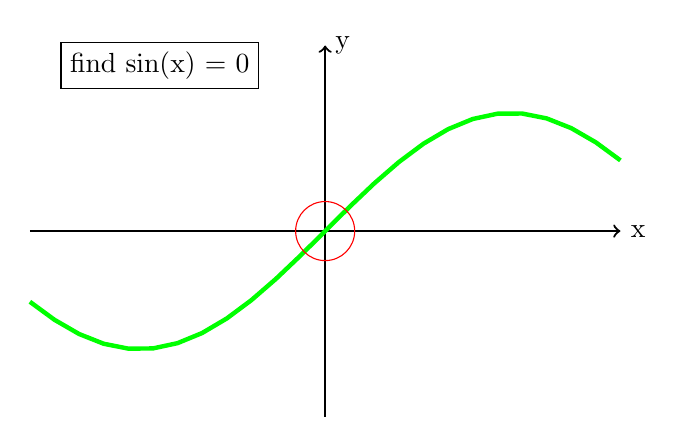
\begin{tikzpicture}[xscale=1.5,yscale=1.5]
    \node[draw] at (-1.4,1.4) {find sin(x) = 0};
    \draw[thick,->] (-2.5,0) -- (2.5,0) node[right]{x};
  \draw[thick,->] (0,-pi/2) -- (0,pi/2) node[right]{y};
    \draw[green, ultra thick,domain=-2.5:2.5] plot (\x, {sin(deg(\x))});
    \draw[red] (0,0) circle (0.25);
    \end{tikzpicture}
}
\subfigure[][The red line shows the location of the initial guess for {$x$}.]{
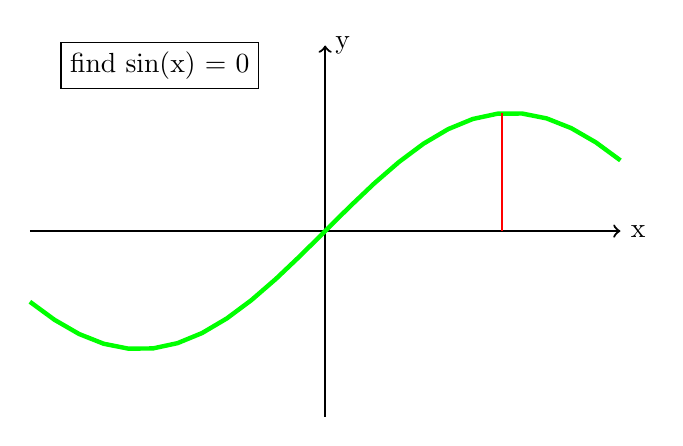
\begin{tikzpicture}[xscale=1.5,yscale=1.5]
    \node[draw] at (-1.4,1.4) {find sin(x) = 0};
    \draw[thick,->] (-2.5,0) -- (2.5,0) node[right]{x};
  \draw[thick,->] (0,-pi/2) -- (0,pi/2) node[right]{y};
    \draw[green, ultra thick,domain=-2.5:2.5] plot (\x, {sin(deg(\x))});
    \draw [red, thick] (1.5,0) -- (1.5,1);
    \end{tikzpicture}
}
\caption{\it A graph of the nonlinear function {$\sin(x)=0$} we are trying to solve.}
\end{figure}

\paragraph{The full Picard iteration}

The full Picard iteration can be written down as $x_{n+1} = f(x_{n})$. For our example, 
that would be $x_{n+1} = \sin(x_{n})$. Solving this nonlinear system through the full Picard 
iteration can be visualized drawing a line $x = y$, as shown in figure 
\ref{fig:cnss-fig2-sin0-full-picard}a. The next $x$ can now be easily found by just graphing 
the value from $sin(1)$ to $x = y$, as can be seen in figure \ref{fig:cnss-fig2-sin0-full-picard}b-d.

The important thing to notice here is that the iteration converges quickly in the beginning, 
but the iteration slows down conciderably, the closer it gets to the solution. It is also 
impotant to note that if there is a single solution, this iteration will almost always 
converge to it. That means it is a very stable, but slow iteration after some iterations. 

In the context of \aspect{} the iteration is usually written as 
\begin{align}
    x_{n+1} = A(x_n)^{-1}b
\end{align}. Because it looks very much like equation \ref{sec:cnss:eq1:axb}, it is usually 
very easy to implement. It only requires a loop over the current linear solve, feeding 
the current solution as the new guess.

\begin{figure}
    \label{fig:cnss-fig2-sin0-full-picard}
\subfigure[][Continuation from figure \ref{fig:cnss-fig1-sin0}b, where 
the black line indicates {$x=y$}]{
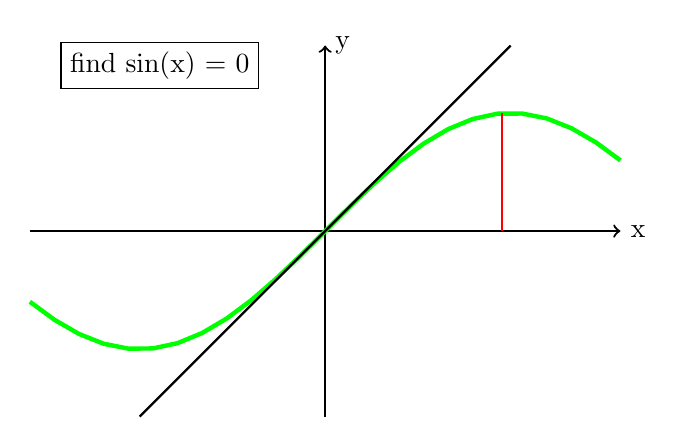
\begin{tikzpicture}[xscale=1.5,yscale=1.5]
    \node[draw] at (-1.4,1.4) {find sin(x) = 0};
    \draw[thick,->] (-2.5,0) -- (2.5,0) node[right]{x};
  \draw[thick,->] (0,-pi/2) -- (0,pi/2) node[right]{y};
    \draw[green, ultra thick,domain=-2.5:2.5] plot (\x, {sin(deg(\x))});
    \draw[black,thick,domain=-pi/2:pi/2] plot (\x,\x) ;
    \draw [red, thick] (1.5,0) -- (1.5,1);
    \end{tikzpicture}
}
    \subfigure[][Red and blue lines show one nonlinear iteration extra compared to figure a.]{
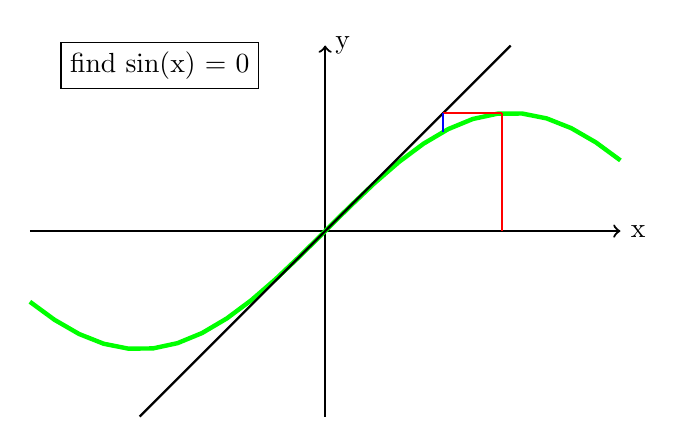
\begin{tikzpicture}[xscale=1.5,yscale=1.5]
    \node[draw] at (-1.4,1.4) {find sin(x) = 0};
    \draw[thick,->] (-2.5,0) -- (2.5,0) node[right]{x};
  \draw[thick,->] (0,-pi/2) -- (0,pi/2) node[right]{y};
    \draw[green, ultra thick,domain=-2.5:2.5] plot (\x, {sin(deg(\x))});
    \draw[black,thick,domain=-pi/2:pi/2] plot (\x,\x) ;
    \draw [red, thick] (1.5,0) -- (1.5,1);
    \draw [red, thick] (1.5,1) -- (1,1);
    \draw [blue, thick] (1,1) -- (1,0.84147);
    \end{tikzpicture}
}
\subfigure[][Red and blue line show one nonlinear iteration extra compared to figure b.]{
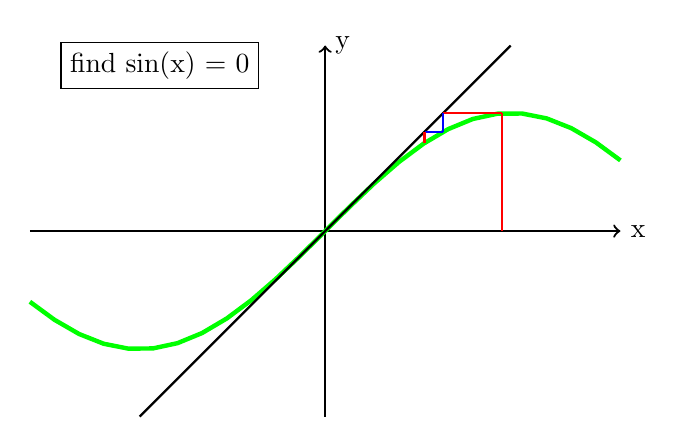
\begin{tikzpicture}[xscale=1.5,yscale=1.5]
\node[draw] at (-1.4,1.4) {find sin(x) = 0};
\draw[thick,->] (-2.5,0) -- (2.5,0) node[right]{x};
\draw[thick,->] (0,-pi/2) -- (0,pi/2) node[right]{y};
\draw[green, ultra thick,domain=-2.5:2.5] plot (\x, {sin(deg(\x))});
\draw[black,thick,domain=-pi/2:pi/2] plot (\x,\x) ;
\draw [red, thick] (1.5,0) -- (1.5,1);
\draw [red, thick] (1.5,1) -- (1,1);
\draw [blue, thick] (1,1) -- (1,0.84147);
\draw [blue, thick] (1,0.84147) -- (0.84147,0.84147);
\draw [red, thick] (0.84147,0.84147) -- (0.84147,0.7456);
\end{tikzpicture}
}
\subfigure[][Red and blue line show one nonlinear iteration extra compared to figure c.]{
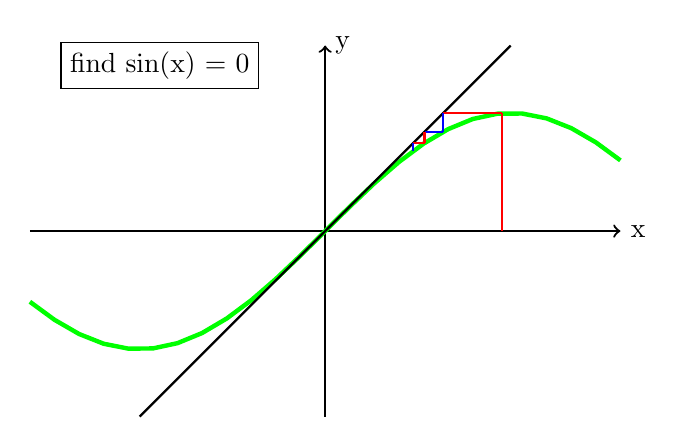
\begin{tikzpicture}[xscale=1.5,yscale=1.5]
\node[draw] at (-1.4,1.4) {find sin(x) = 0};
\draw[thick,->] (-2.5,0) -- (2.5,0) node[right]{x};
\draw[thick,->] (0,-pi/2) -- (0,pi/2) node[right]{y};
\draw[green, ultra thick,domain=-2.5:2.5] plot (\x, {sin(deg(\x))});
\draw[black,thick,domain=-pi/2:pi/2] plot (\x,\x) ;
\draw [red, thick] (1.5,0) -- (1.5,1);
\draw [red, thick] (1.5,1) -- (1,1);
\draw [blue, thick] (1,1) -- (1,0.84147);
\draw [blue, thick] (1,0.84147) -- (0.84147,0.84147);
\draw [red, thick] (0.84147,0.84147) -- (0.84147,0.7456);
\draw [red, thick] (0.84147,0.7456) -- (0.7456,0.7456);
\draw [blue, thick] (0.7456,0.7456) -- (0.7456,0.6784);
\end{tikzpicture}
}
\caption{A visualization of the full Picard iteration for the nonlinear function {$\sin(x)=0$}.}
\end{figure}

\paragraph{The Newton iteration}

The Newton iteration can be written down as $x_{n+1} = x_n - \frac{f(x_n)}{f'(x_n)}$. This means  
that we are mostly interested in computing an update to the current solution. To compute the 
update we not only need to calculate $f(x_n)$, but also the derivative $f'(x_n)$. The iteration 
can be visualized in the same way as the Picard iteration, but we won't need the line $x=y$ 
anymore, and we will start from a slightly different starting guess: $x=1$. The reason for
starting from a slightly different starting guess will hopefully become clear soon. The 
deriative at $x=1$ is $\cos(1)$, so the new $x_{n+1}$ becomes $1-\frac{\sin(1)}{\cos(1)}=-0.557$. 

There are a few things that are important to notice in figure \ref{fig:cnss-fig3-sin0-Newton}. 
First, in practice each iteration can be represented as a vector with
the origin at the solution of $(x,\sin(x))$ pointing in the direction of the derivative. This 
means that this vector has a certain length, which we will get back to later.
Second, when the iteration converges, it can do so much faster than the Picard 
iteration (see subfigures a and b). Third, when the initial guess
is too far from the solution, the updated guess maybe further away from the solution (figure 
\ref{fig:cnss-fig3-sin0-Newton}d). A special case of this is when the derivative is zero 
(figure \ref{fig:cnss-fig3-sin0-Newton}c). Both figure  \ref{fig:cnss-fig3-sin0-Newton}c and d
visually show why it is important for the Newton iteration to have a good starting guess. 
Some strategies to achieve this, also called globalization, will be discussed in section 
\ref{sec:cnns:globalization}.


\begin{figure}
    \label{fig:cnss-fig3-sin0-Newton}
\subfigure[][Continuation from figure \ref{fig:cnss-fig1-sin0}b, with starting
guess {$x=1$} and the derivative of that $x$ plotted.]{
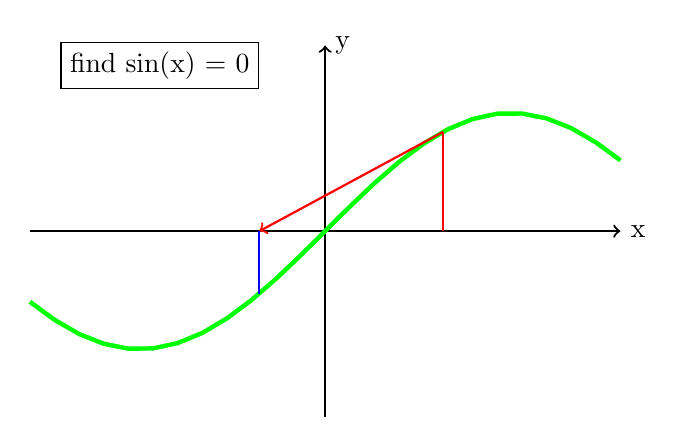
\begin{tikzpicture}[xscale=1.5,yscale=1.5]
    \node[draw] at (-1.4,1.4) {find sin(x) = 0};
    \draw[thick,->] (-2.5,0) -- (2.5,0) node[right]{x};
  \draw[thick,->] (0,-pi/2) -- (0,pi/2) node[right]{y};
    \draw[green, ultra thick,domain=-2.5:2.5] plot (\x, {sin(deg(\x))});
    \draw[red, thick, domain=-pi:pi] (1,0) -- (1,0.84147);
    \draw[red,thick, <-, domain=-0.5574:1.0] plot (\x,0.54*\x+0.30);
    \draw[blue, thick, domain=-pi:pi] (-0.5574,0) -- (-0.5574,-0.5290);
    \end{tikzpicture}
}
\subfigure[][Continuation from figure a, with the blue and red lines showing 
one more iteration.]{
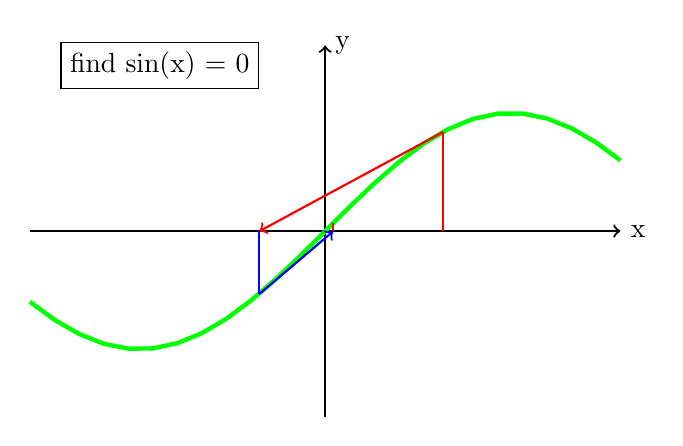
\begin{tikzpicture}[xscale=1.5,yscale=1.5]
    \node[draw] at (-1.4,1.4) {find sin(x) = 0};
    \draw[thick,->] (-2.5,0) -- (2.5,0) node[right]{x};
  \draw[thick,->] (0,-pi/2) -- (0,pi/2) node[right]{y};
    \draw[green, ultra thick,domain=-2.5:2.5] plot (\x, {sin(deg(\x))});
    \draw[red, thick, domain=-pi:pi] (1,0) -- (1,0.84147);
    \draw[red,thick, <-, domain=-0.5574:1.0] plot (\x,0.54*\x+0.30);
    \draw[blue, thick, domain=-pi:pi] (-0.5574,0) -- (-0.5574,-0.5290);
    \draw[blue, thick,->,domain=-0.5574:0.0659] plot (\x,0.8486*\x-0.06);
    \draw[red, thick, domain=-pi:pi] (0.0659,0) -- (0.0659,0.0658);
    \end{tikzpicture}
}

\subfigure[][Same as figure a, but now showing the case where the initial guess
leads to a derivative which is zero. This will lead to a division by zero, in the
update and the solution will be undefined. For a system of equations, the linear
solver should fail.]{
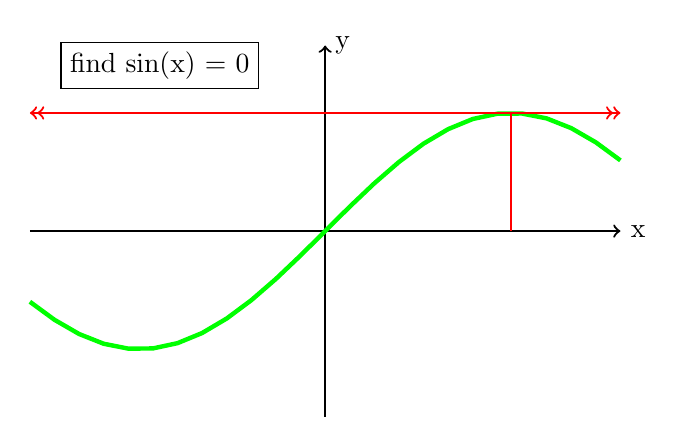
\begin{tikzpicture}[xscale=1.5,yscale=1.5]
    \node[draw] at (-1.4,1.4) {find sin(x) = 0};
    \draw[thick,->] (-2.5,0) -- (2.5,0) node[right]{x};
  \draw[thick,->] (0,-pi/2) -- (0,pi/2) node[right]{y};
    \draw[green, ultra thick,domain=-2.5:2.5] plot (\x, {sin(deg(\x))});
    \draw[red, thick, domain=-pi:pi] (pi/2,0) -- (pi/2,1);
    \draw[red,thick,<<->>, domain=-1.4:1] (-2.5,1) -- (2.5,1);
    \end{tikzpicture}
}
\subfigure[][Same as figure a, but now showing the case where the initial guess is further away.
In this case the direction of the next update will be further away from the solution and the
iteration will diverge.]{
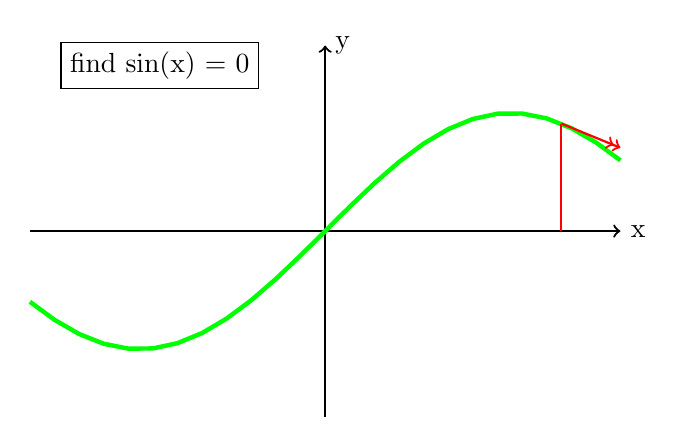
\begin{tikzpicture}[xscale=1.5,yscale=1.5]
    \node[draw] at (-1.4,1.4) {find sin(x) = 0};
    \draw[thick,->] (-2.5,0) -- (2.5,0) node[right]{x};
  \draw[thick,->] (0,-pi/2) -- (0,pi/2) node[right]{y};
    \draw[green, ultra thick,domain=-2.5:2.5] plot (\x, {sin(deg(\x))});
    \draw[red, thick, domain=-pi:pi] (2,0) -- (2,0.909);
    \draw[red,thick, ->>, domain=2:2.5] plot (\x,-0.41*\x+1.73);
    \end{tikzpicture}
}
\caption{A visualization of the Newton iteration for the nonlinear function {$\sin(x)=0$}.}
\end{figure}


For the Newton iteration, the equation is usually written as 
\begin{align}
    \label{sec:cnss:eq3:JdxAxx-b}
    J \delta x &= A(x) x - b \\
    &= -F
\end{align}. In this equation, the right hand side (rhs) ($A(x)x-b$ or $-F$) will be exactly 
zero when $x$ is the exact solution to the nonlinear problem. Therefore this is also called the 
residual. $J$ is called the Jacobian, which is a derivative matrix. In our simple example, 
this would just be the derivative. So we solve for $\delta x$ now instead of $x$:

\begin{align}
    \delta x_n &= J^{-1}\left(A(x_n) x_n - b\right)
\end{align}. Next we can compute the new solution with $x_{n+1} = x_n - \delta x_n$. This 
form of computing an update/correction to the solution instead of computing the full
solution every time is called a defect correction scheme.

For reasons beyond the scope of this cookbook, depending on the rheology model, the Jacobian 
matrix may sometimes be the equivalent of figure \ref{fig:cnss-fig3-sin0-Newton}, which 
means that the linear solver will fail. To stabilize this, there are some stabilization 
options available in ASPECT based on \cite{FBTGS19}, of which the most important is the 
SPD option. When you need to choose, it is important to know that the unstabilized version
will always converge at the same speed or faster than the stabilized version. Theoretically 
this means that you will only want to stabilize when needed. This is an option for the Newton
solver called the fail-safe. With the fail-safe you can run an unstabilized version of 
the Newton iteration, and when the linear solver fails, it will automatically turn on all
the stabilizations for the rest of the timestep and retry the nonlinear iteration. The downside
is that it may take a long time for the linear solver to fail, especially if it fails every
timestep. So if you know that the model you are using is causing the linear solver to always
fail, it is faster to just always turn on the stabilization.
Note that the stabilization only works properly for the incompressible case.


\paragraph{Defect correction Picard iteration}

The last iteration scheme, the defect correction Picard iteration, is mathematically 
equivalent to the Picard iteration, but written in the form of the Newton solver. It 
turns out that the Jacobian in equation \ref{sec:cnss:eq3:JdxAxx-b} internally consists
of two parts: 
\begin{align}
    \label{sec:cnss:eq4:JxAxApx}
    J(x) = A(x) + A'(x) 
\end{align}. If we approximate the Jacobian by setting it 
equal to $A(x)$, the iteration will converge like a Picard iteration. The only difference 
is that computationally this defect correction form is more precise while requiring a less strict
linear tolerance. This can speed up your computation and may help slightly with convergence
in some cases. 

\paragraph{Globalization of the Newton iteration}
\label{sec:cnns:globalization}

\subparagraph{Switch between the Picard and Newton iteration}
One of the easiest globalization strategies for the Newton solver is to first do a few
Picard iterations. Remember that the Picard iteration will practically always converge 
(although for single iterations the residual may go up, the trend is usually down). Once
you are close enough to the solution, switching to the Newton solver should than make 
the iteration converge quickly. The main issue is knowing when you are close enough to 
the solution so that the Newton solver works well. Unfortunately this is problem dependent,
but a combination between the different globalization options in this section should help.

\subparagraph{Transition between the Picard and Newton iteration}
The change between the Picard and Newton iteration does not have to be a hard switch. 
When looking at equation \ref{sec:cnss:eq4:JxAxApx}, we can introduce a variable $c_k$
and multiply it with $A'(x)$:
\begin{align}
    J(x) = A(x) + c_k A'(x) 
\end{align}. When $c_k$ is zero, the iteration behaves like a Picard iteration and when 
it is one, it behaves like a Newton iteration. In \aspect{} we have implemented an option, 
which we refer to as the Residual Scaling Method(RSM). If enabled, this automatically 
computes $c_k = \max\left(0.0,1.0-\frac{r_k}{r_{N_{DC}}}\right)$, where $r_k$ 
is the current nonlinear residual and $r_{N_{DC}}$ is the residual in the first iteration 
after switching to the Newton method. This option allows to more gradually switch to the 
Newton interation and also gradually switch back if the iteration diverges. 

\subparagraph{Line search}
The idea behind the line search is to check whether when applying the update to the 
solution, the residual has gotten smaller. If the residual has not gotten sufficiently 
smaller, then it scales the update such that it is smaller until the next residual is 
sufficiently smaller than the current residual.

\paragraph{Some practical tips}
The Newton solver is a complex solver with many options, and without a bit of testing may 
actually be slower than using a Picard iteration. This may even be the case if it takes 
less iterations, since computing the derivatives for the Newton iteration can be expensive.

Always start with running a representative model with just a defect correction Picard iteration.
Note that the defect correction Picard and the Newton method work well with much lower 
linear solver tolerances. A value of $1e-2$ is a good default, but you may be able to 
even use $1e-1$. 
If the nonlinear residual doesn't converge quickly enough or at all to the desired nonlinear 
tolerance, then it is time to consider using the full Newton solver. It is strongly 
recommended to start by plotting the convergence behavior of the defect correction Picard 
method, with number of nonlinear iterations on the x axis and the nonlinear residual on a 
logscale y axis. This will allow you to see the convergence behavior much more clearly 
than by just looking at the numbers in the \aspect{} output file. Furthermore, it allows 
for a much better comparison with the convergence behavior of the Newton solver and 
between different settings of the Newton solver. For examples of such plots and more advice, 
please see section 3 of \cite{FBTGS19}.